\section{Model order selection}

We have defined the models as:
\[\mathcal{M}(\vartheta)=\left\{ M(\vartheta),\vartheta \in \Theta \subseteq \mathbb{R}^{n_\theta}\right\}\]
This representation constitutes a fixed-order model class, implying that we cannot guarantee  $\mathcal{S} \in \mathcal{M}(\vartheta)$. 
It's important to note that we lack a method to expand $\mathcal{M}(\vartheta)$ if the system lies outside it.

For simplicity, let's assume $n_\theta=n=m=p$, meaning a single parameter describes the model order.
The process for selecting the parameter $n_\theta$ begins by choosing an initial value and incrementing it if necessary, up to a maximum of $n_{\text{max}}$:
\begin{algorithm}[H]
    \caption{Model order selection algorithm}
        \begin{algorithmic}[1]
            \State $n \leftarrow 1$
            \Repeat 
                \State $\mathcal{M}(\vartheta)\leftarrow\left\{ M(\vartheta),\vartheta \in \Theta \subseteq \mathbb{R}^{n_\theta}\right\}$
                \State $\hat{\vartheta}_N^{(n)} \leftarrow \argmin_{\vartheta} J_N(\vartheta)$
            \Until $n=n_{max}$
        \end{algorithmic}
\end{algorithm}
As the model order increases, the total cost decreases.
When we achieve a total cost of approximately $\lambda^2$, we have reached the optimal order for the selected model.

Overfitting occurs with increased order, eventually leading to a cost of zero. 
This happens when $n_\vartheta=N$.
\begin{figure}[H]
    \centering
    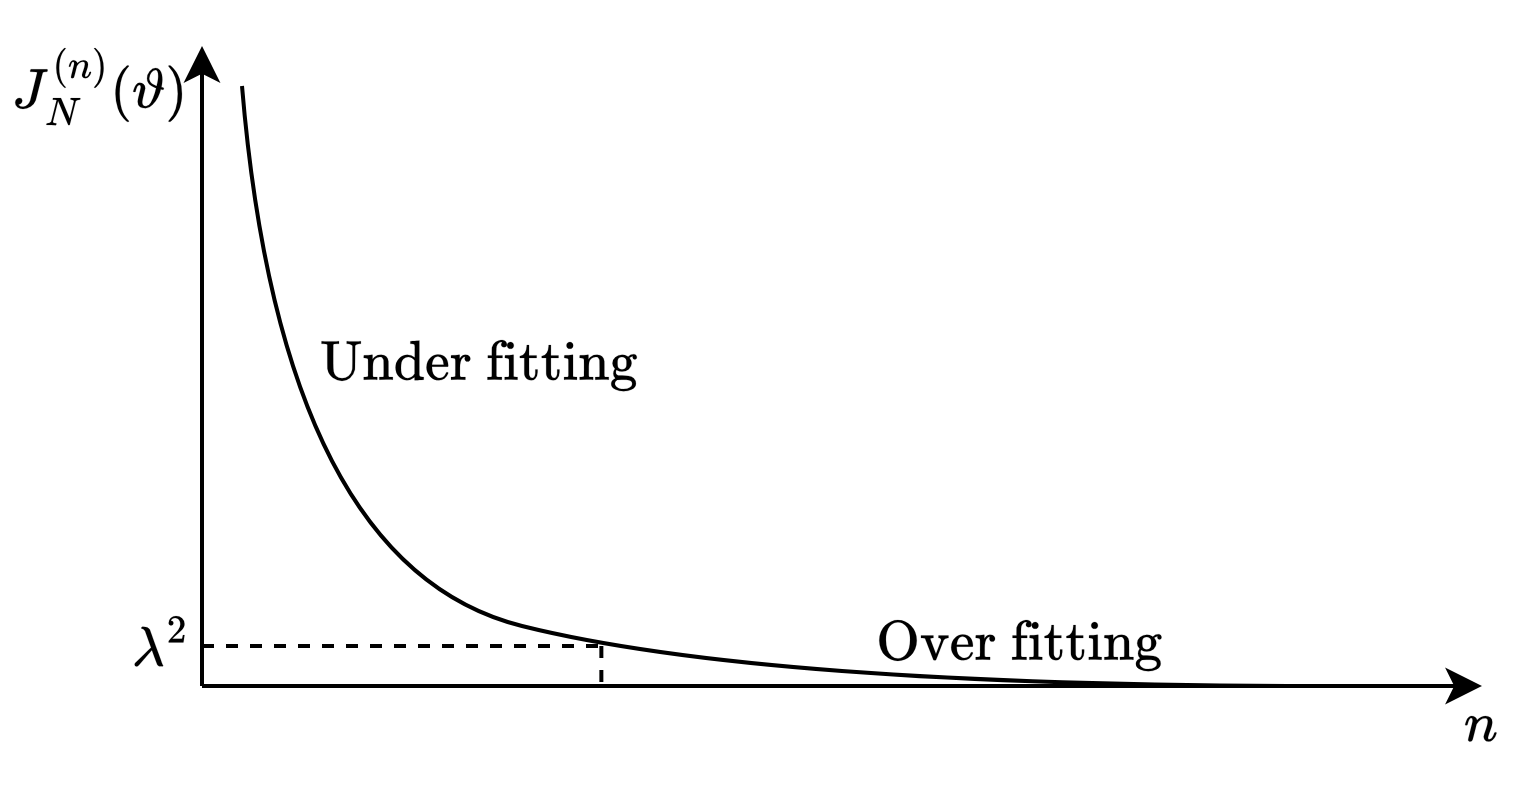
\includegraphics[width=0.6\linewidth]{images/fitting.png}
    \caption{Cost function with respect to the order}
\end{figure}
However, this method isn't ideal because the value of $\lambda^2$ is generally unknown.
Possible alternatives include:
\begin{enumerate}
    \item Whiteness test on residuals.
    \item Cross-validation.
    \item Identification with model order penalties.
\end{enumerate}

\subsection{Whiteness test on residuals}
We understand that if $\mathcal{S} \in \mathcal{M}(\vartheta)$ for a certain $n$, then $\hat{\vartheta}_N^{(n)} \approx \vartheta^\circ$ and $\varepsilon(t,\hat{\vartheta}_N^{(n)})\approx e(t)$, where $\varepsilon(t,\hat{\vartheta}_N^{(n)})$ approximates  White Noise.

To determine the appropriate model order $n$, we assess whether $\varepsilon(t,\hat{\vartheta}_N^{(n)})$ exhibits whiteness. 
We select the first $n$ for which the whiteness test yields favorable results.

The whiteness test typically involves a covariance check, which should be non-zero at $\tau=0$ and zero otherwise. 
Alternatively, a spectral density check can be performed:  White Noise exhibits a constant spectrum value.

\paragraph*{Problems}
The limitation of this method arises from the fact that the covariance at time instants other than zero may vary, making it challenging to determine whether a process exhibits  White Noise characteristics.
Similarly, the spectral check may show slight variations across different instants instead of a perfectly horizontal line.
\begin{figure}[H]
    \centering
    \begin{subfigure}{0.49\textwidth}
        \centering
        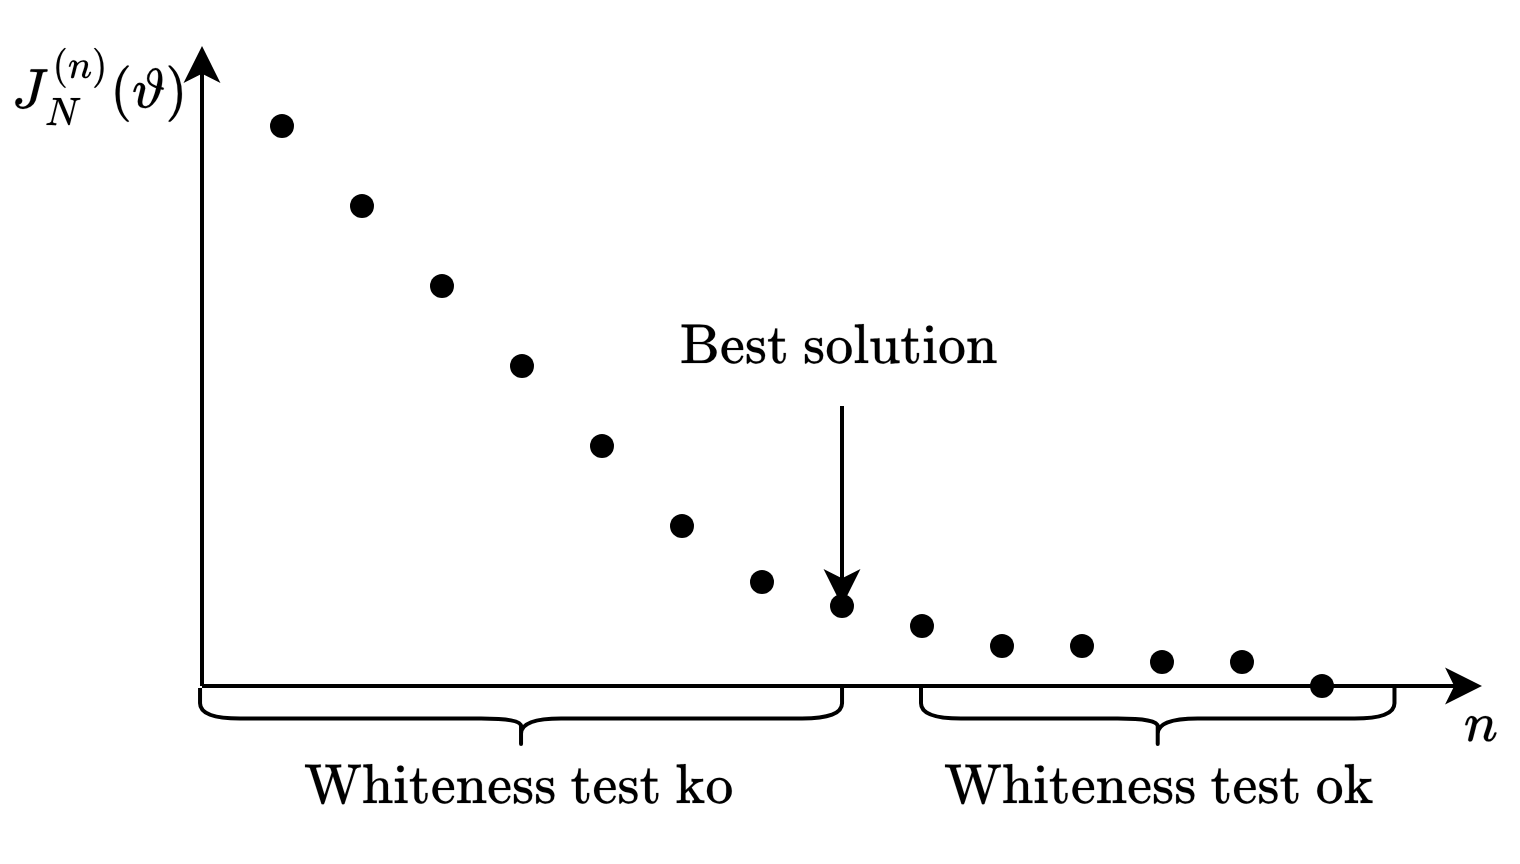
\includegraphics[width=0.9\linewidth]{images/wone.png} 
        \caption{Ideal situation}
    \end{subfigure}
    \begin{subfigure}{0.49\textwidth}
        \centering
        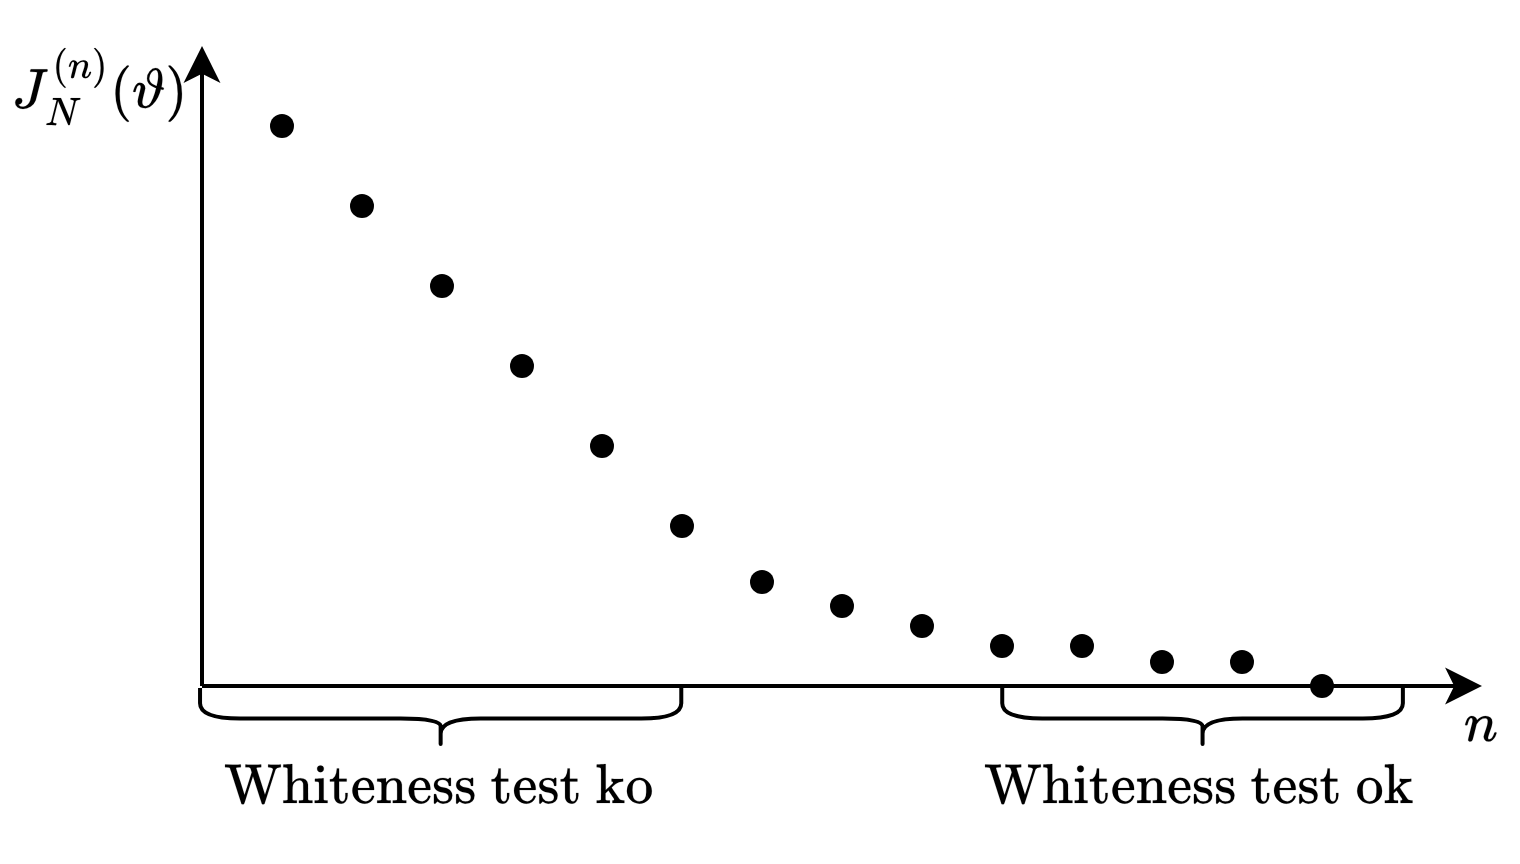
\includegraphics[width=0.9\linewidth]{images/wtwo.png}
        \caption{Real situation}
    \end{subfigure}
    \caption{Whiteness test outcomes}
\end{figure}
In the real scenario, we can narrow down the set of candidate model orders, but identifying the exact order remains challenging.

\subsection{Cross-validation}
Let's consider a scenario where we have a total of $N$ data points, which we divide into two halves:
\begin{itemize}
    \item Identification dataset: $\left\{ y(1),y(2),\dots,y(\frac{N}{2}) \right\}$. 
    \item Validation dataset: $\left\{ y\left(\frac{n}{2}+1\right),y\left(\frac{n}{2}+2\right),\dots,y(N) \right\}$. 
\end{itemize}
\begin{algorithm}[H]
    \caption{Model order selection algorithm}
        \begin{algorithmic}[1]
            \For {$n=1$ \textbf{to} $n=n_{max}$}
                \State find $\hat{\vartheta}_{N/2}\leftarrow\argmin_{\vartheta} J_N(\vartheta)=\argmin_{\vartheta}\frac{1}{N/2}\sum_{t=1}^{N/2}\left( y(t)-\hat{y}(t|t-1,\vartheta) \right)^2$
                \State evaluate $J_V\left(\hat{\vartheta}_{N/2}^{(n)}\right) \leftarrow \frac{1}{N/2}\sum_{t=n/2+1}^{N}\left( y(t)-\hat{y}(t|t-1,\hat{\vartheta}_{N/2}^{(n)}) \right)^2$
            \EndFor
            \State choose $n$ minimizing $J_V$
        \end{algorithmic}
\end{algorithm}
Note that the $\frac{N}{2}$ used in the evaluation step is not the same as the $\frac{N}{2}$ used in the preceding step. 
This distinction is important because, in the evaluation step, we only consider the second portion of the available $N$ data using the value of $\hat{\vartheta}_N$ found with the other half of the data. 
We then compute the variance of the prediction error in the second dataset.

The difference between the costs computed on the whole dataset and half of it is significant. 
In the former case, the cost keeps decreasing, while in the latter, it initially decreases and then rises again.
\begin{figure}[H]
    \centering
    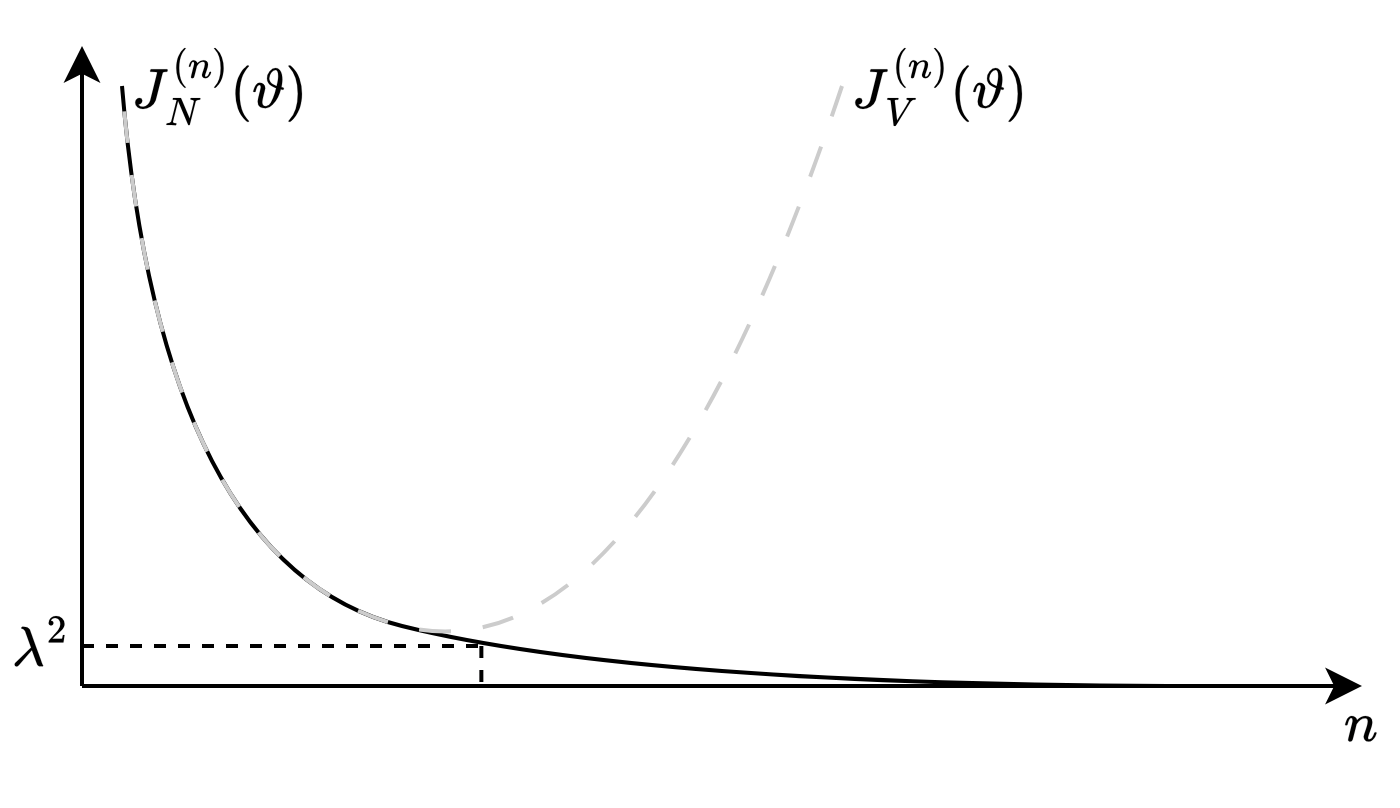
\includegraphics[width=0.54\linewidth]{images/fitting1.png}
    \caption{Difference between the cost functions $J_N$ and $J_V$}
\end{figure}

\paragraph*{Problems}
The primary challenge associated with this method is the requirement for many elements in the initial dataset $N$ to ensure sufficient data in the considered half.

\subsection{Identification with model order penalties}
When the dataset's size is insufficient, identification with model order penalties becomes impractical. 
Unlike cross-validation, where the same cost is applied to different data, the penalized-cost approach employs a distinct cost on the same dataset.

Instead of minimizing $J_N(\vartheta)$ directly, we aim to minimize one of the following measures:
\begin{itemize}
    \item \textit{Final prediction error}: we seek to minimize $\mathbb{E}[J_N(\vartheta)]$ with respect to noise realizations. 
        As computing the expected value directly isn't feasible, we minimize the final prediction error:
        \[\text{FPE}(n)=\dfrac{N+n}{N-n}J_N\left(\hat{\vartheta}_N^{(n)}\right)\]
        \begin{figure}[H]
            \centering
            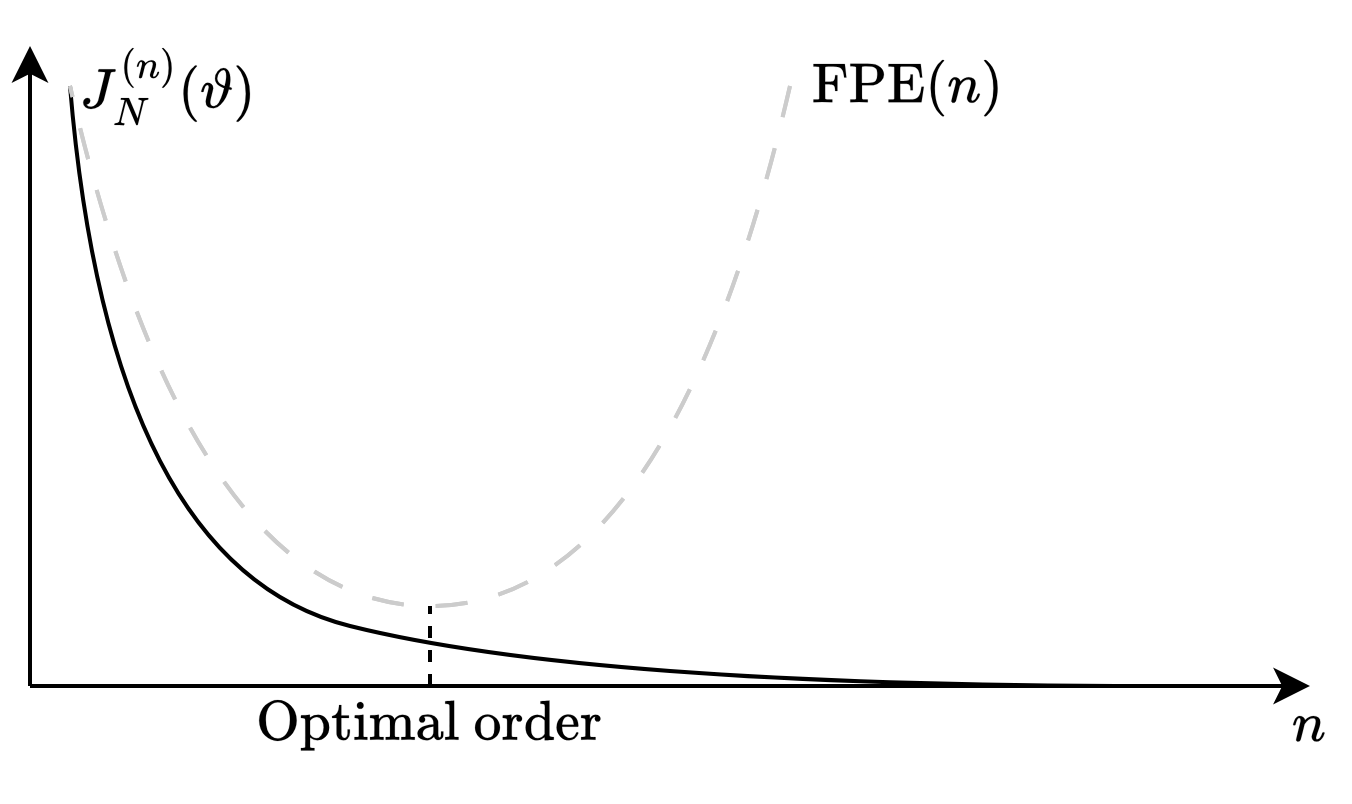
\includegraphics[width=0.54\linewidth]{images/fpe.png}
            \caption{Difference between the cost functions $J_N$ and and final prediction error}
        \end{figure}
    \item \textit{Akaike information criterion}:
        \[\text{AIC}(n)=\ln \left( J_N(\hat{\vartheta}_N^{(n)}) \right)+2\dfrac{n}{N}\]
        The penalty on the current order $n$ increases with $n$, while the cost decreases as the order increases. 
        Balancing these two components is crucial for optimal results.
    \item \textit{Minimum description length}: 
        \[\text{MDL}(n)=\ln \left( J_N(\hat{\vartheta}_N^{(n)})\right)+\ln(N)\dfrac{n}{N}\]
        Minimum description length operates similarly to Akaike information criterion.
\end{itemize}

\paragraph*{FPE and AIC}
We begin with:
\begin{align*}
    \ln(\text{FPE}) &= \ln\left( \dfrac{N+n}{N-n}J_N\left(\hat{\vartheta}_N^{(n)}\right) \right) \\
                    &= \ln\left( \dfrac{1+\frac{n}{N}}{1-\frac{n}{N}}J_N\left(\hat{\vartheta}_N^{(n)}\right)\right) \\
                    &= \ln\left(1+\frac{n}{N}\right) - \ln\left(1-\frac{n}{N}\right) + \ln\left(J_N\left(\hat{\vartheta}_N^{(n)}\right)\right)
\end{align*}
Given that $\frac{n}{N}$ is usually small, we approximate:
\begin{align*}
    \ln(\text{FPE}) &= \ln\left(1+\frac{n}{N}\right) - \ln\left(1-\frac{n}{N}\right) + \ln\left(J_N\left(\hat{\vartheta}_N^{(n)}\right)\right) \\
                    &= \frac{n}{N} - \left(-\frac{n}{N}\right) + \ln\left(J_N\left(\hat{\vartheta}_N^{(n)}\right)\right) \\
                    &= 2\frac{n}{N} + \ln\left(J_N\left(\hat{\vartheta}_N^{(n)}\right)\right) \\
                    &= \text{AIC}(n)
\end{align*}
Thus, both methods yield the same information criterion. 
Consequently, minimizing one metric also minimizes the other.

\paragraph*{AIC and MDL}
The primary distinction between the Akaike Information Criterion (AIC) and Minimum Description Length (MDL) lies in the coefficient of the penalty term. 
AIC maintains a fixed penalty value of two, while MDL incorporates a variable term $\ln(N)$.

Consequently, if $\ln(N) > 2$, indicating $N > 8$, MDL penalizes the model order more severely than AIC.

In cases where $\mathcal{S} \in \mathcal{M}(\vartheta)$ and $\mathcal{M}(\vartheta)$ represents the set of ARX models, MDL is the preferred choice. 
However, in general scenarios where $\mathcal{S} \notin \mathcal{M}(\vartheta)$, a slight overfitting is acceptable, making AIC the preferred criterion.